\typeout{comp551 writeup template}

% These are the instructions for authors for IJCAI-19.

\documentclass[11pt]{article}
\pdfpagewidth=8.5in
\pdfpageheight=11in
\usepackage{comp551}

% Use the postscript times font!
%\usepackage{times}
\usepackage{graphicx}
\usepackage{soul}
\usepackage{url}
\usepackage[hidelinks]{hyperref}
\usepackage[utf8]{inputenc}
\usepackage[small]{caption}
\usepackage{graphicx}
\usepackage{amsmath}
\usepackage{booktabs}
\urlstyle{same}

% the following package is optional:
\usepackage{latexsym} 

\title{MiniProject 1: Predicting the Popularity of Reddit Comments using Linear Regression}

\author{%
\begin{tabular}{c} Jean-Sébastien Grondin \\ \normalfont McGill Id:260345519  \\ \normalfont \small jean-sebastien.grondin@mail.mcgill.ca \end{tabular} 
\begin{tabular}{c} Zhourong Li \\ \normalfont McGill Id:260674414  \\ \normalfont \small zhourong.li@mail.mcgill.ca \end{tabular} 
\begin{tabular}{c} Zhenze Han \\ \normalfont McGill Id:260675404  \\ \normalfont \small zhenze.han@mail.mcgill.ca \end{tabular} }

\begin{document}

\maketitle

\begin{abstract}
This paper presents the methodology and results obtained when predicting the popularity of Reddit comments using linear regression. This study used a dataset of 12000 instances which was split into training, validation and test sets.  Several additional features were extracted and analyzed for improving the model performance. \textbf{We found that...} The model achieved a mean squared error (MSE) of  \textbf{X.XXX} on the test set. 
\end{abstract}

\section{Introduction}
Reddit is a popular social media site which is currently the 5th most popular website in the United States according to Alexa. It is essentially a massive collection of forums and threads where users can upvote or downvote comments that they like or dislike (see an example below).\\
\\

\includegraphics[width=8cm]{reddit}\\
\\
The objective of this study was to implement and evaluate a linear regression model for predicting the popularity score of Reddit comments. A total of 12000 instances of text comments were available, in addition to other features such as the controversiality score and the number of replies each comment received. Text comments were processed in order to extract a word count occurence feature for the most frequently occuring words. Several other features were generated, and the two features which exhibited the highest correlation with the popularity score were retained. Both the closed form and the gradient descent solutions were implemented and compared. The mean squared error was the metric used for all comparisons and analysis. The closed-form approach was used for subsequent experiments as it was found to be faster and more stable and also because it yields the exact solution. Models which included word occurence features were found to overfit compared to models that did not include word occurence features, so these features were droped from the final model. The two new features that were extracted were shown to improve the model performance without causing overfitting. The final model achieved a mean squared error of \textbf{X.XXX} on the test set. 


\section{Dataset}

The original dataset was obtained from the subreddit community \textbf{r/Askreddit}. The dataset contained 12000 instances  with the following information:

\begin{itemize}
    	\item \textbf{popularity\_score:} This metric indicates how popular each comment is and is computed by Reddit. This is the target variable in this study. 
   	\item \textbf{children:} This feature indicates how many replies each comment received.
    	\item \textbf{is\_root:} This feature is True when a comment is the "root" of a conversation and is False when it is a reply to another comment.
    	\item \textbf{controversiality:} This feature is a binary variable that indicates if a comment is controversial (when equals 1) or not controversial (when equals 0). A controversial comment is one that receives close to the same amount of upvotes and downvotes.
    	\item \textbf{text:} The raw text of each comment.
\end{itemize}

The is\_root boolean values were encoded using 0 and 1.  The dataset was then split into training (80\%), validation (10\%) and test (10\%) sets and the training set was subsequently used for text processing, exploratory data analysis and feature extraction. Simple pre-processing was applied to text comments by first a) lower-casing all text and then b) spliting text based on whitespace tokens to generate a list of all words. A list of the 160 most frequently occurring words in the training data was then computed. For every text comments, a 160-dimensional feature vector, $x_{counts}$, was extracted, with $x_{counts}[i]$ being equal to the number of times the ith most frequent word occured in the comment. Using the same list, word occurence feature vectors were extracted for the test and validation sets. 
\\

Some exploratory data analysis was also achieved. The following figure gives a visual representation of the original non-text features. Several observations were made. The popularity score was found to increase with an increasing number of children. Also, controversial comments generally did not lead to high popularity nor high number of children. While it is not readily noticeable in the plot, the mean popularity score is slightly higher (0.981) for non-root comments compared to root comments (0.703), and the [min, max] range is also shorter [-6.267, 7.981] for non-root comments than for root comments [-6.779, 8.373]. \\
\\
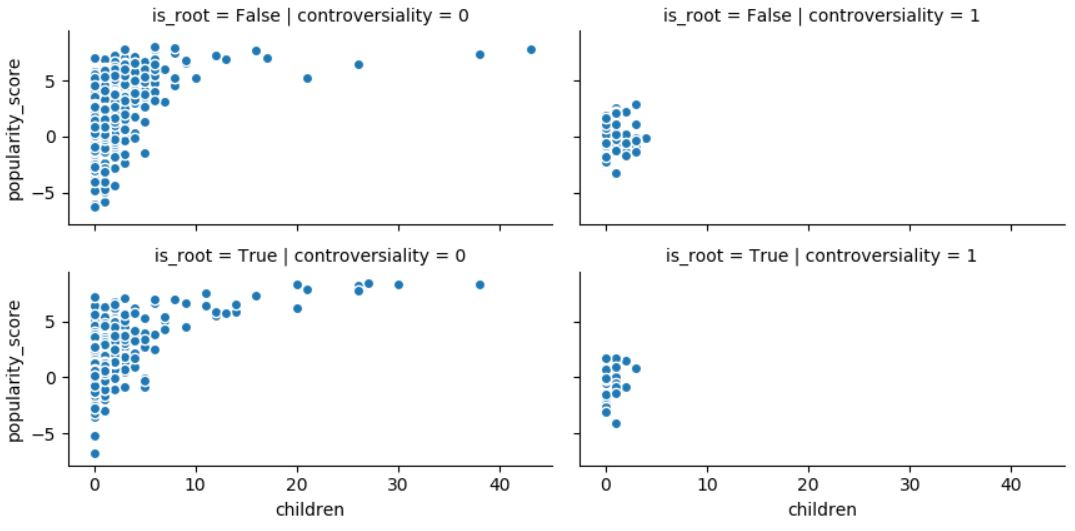
\includegraphics[width=8.5cm, height=6cm]{EDA-1}\\
\\
Since children seemed to be somewhat correlated with the popularity, the following additional features were generated for further analysis: $children^{2}$, $children^{3}$, $ \ln children$, $(\ln children)*(1-controversiality)$. Also, two additional features were also extracted from the text comments: a) the length of each comment and b) the number of exclamation marks occurring in each comment. A correlation matrix heatmap was then computed to assess the correlation of features with the target variable and is displayed below: \\
\\
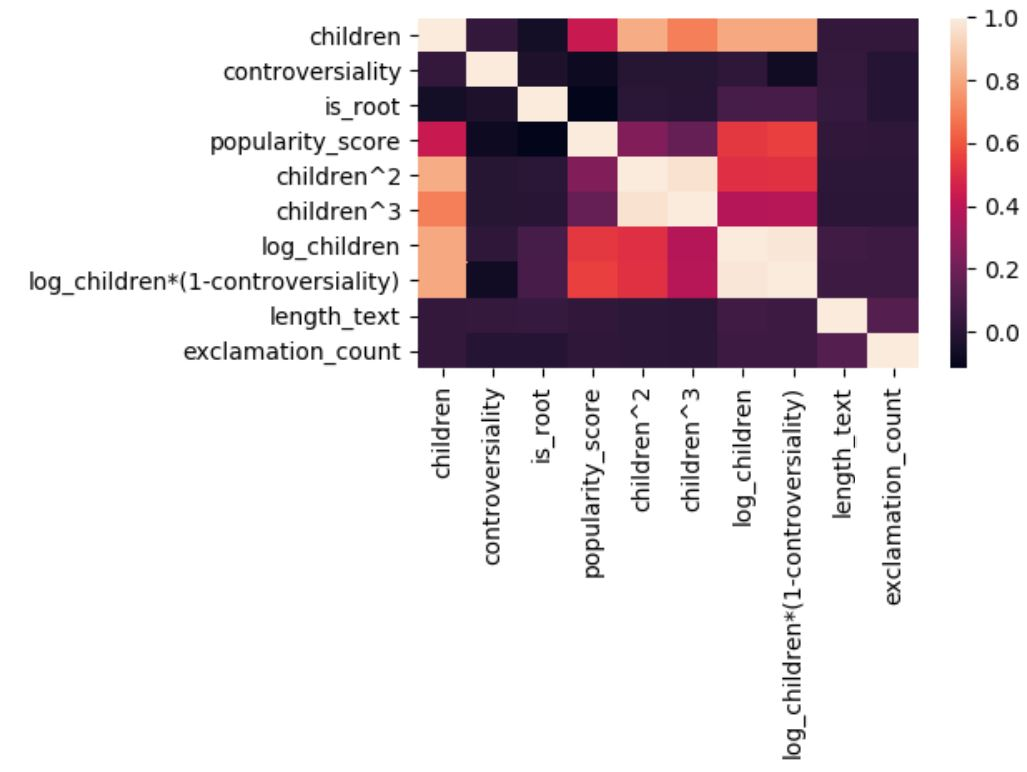
\includegraphics[width=8.5cm, height=6cm]{EDA-4}\\
\\
The two additional text related features mentioned above were not investigated further as they did not seem to be sufficiently correlated to the target variable. As for the others, a discussion of how these contribute to the model performance is included in the following section.\\
\\
Before moving on to the results section, readers should be wary of the ethical implications of using machine learning with social media data for analyzing or filtering information. For example, if machine learning models are used to provide intelligence, they can introduce several types of bias related to the way data is collected, models are built, etc. Hence the authors wish that readers are cautious about a potential misuse of the models or a flawed interpretation of the results. \\
\section{Results}
Following are the results from our test data. Note that the records were based on the performance of an intel i9 processor, so the runtime may vary when using different machines.  For these experiments, the text features are safely ignored as suggested in the instruction, and only using the three features provided.\\
\\
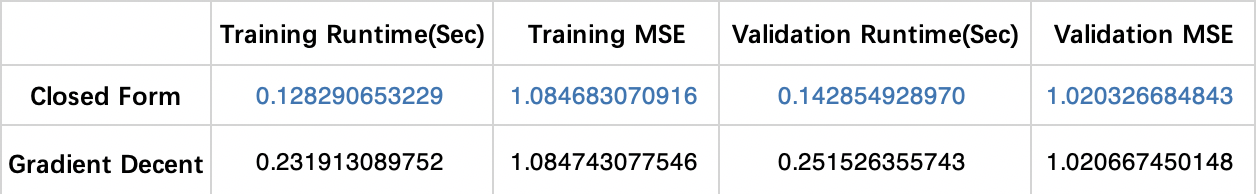
\includegraphics[width=9cm, height=1.5cm]{runtime.png}\\
\\
The table above showing the runtime and MSE of Training Set (Denote as Training in the table, with hyper-parameters: $eta_0$ = 0.000006, $beta$ = 0, $eps$ = 0.0001),  as well as Runtime and MSE of Validation Set (Denote as Validation). The better results are shown in blue. Observe the result we find that, using three features, the closed form approach has smaller running time and attains better MSE in both the Training Sets and Validation Sets. For the gradient decent approach, it takes longer running time, attains slightly poor results. \\
\\
For the stability of two different approaches, the closed form approach is more stable because its value is always fixed, for example, using 3 features, the closed form solution always have the MSE= 0.128290653 for the training set. While for the gradient decent approach, the MSE will be effected by the change of the choosing of hyper parameters: $eta_0$, $beta$, $eps$ and we also found the scaling of the learning rate will also effect the value of MSE.
\newpage
Here we fix $eta_0$ = 0.000006, $eps$ = 0.0001, and change the $beta$ value:\\ 
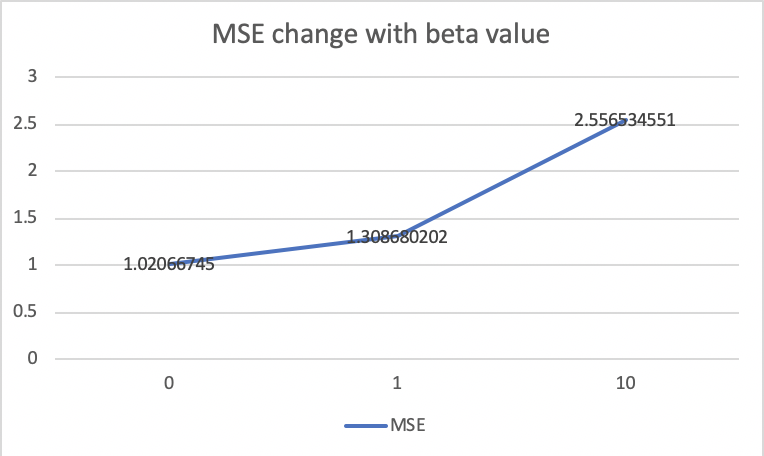
\includegraphics[width=8.5cm, height=6cm]{beta.png}\\
\\
Observe the table we can find the MSE was increasing as the value of $beta$ increasing. Note the $beta$ value are not scaled equally because we just want to emphasize the stability of the gradient decent is not good as closed form approach, and from our test results, $beta$=0 has the smallest MSE value.\\
\\
Now we fix $beta$ = 0, $eps$ = 0.0001 and change the $eta_0$ value, the horizontal axis represents the value of $eta_0$ value, while the vertical axis represents the MSE:\\ 
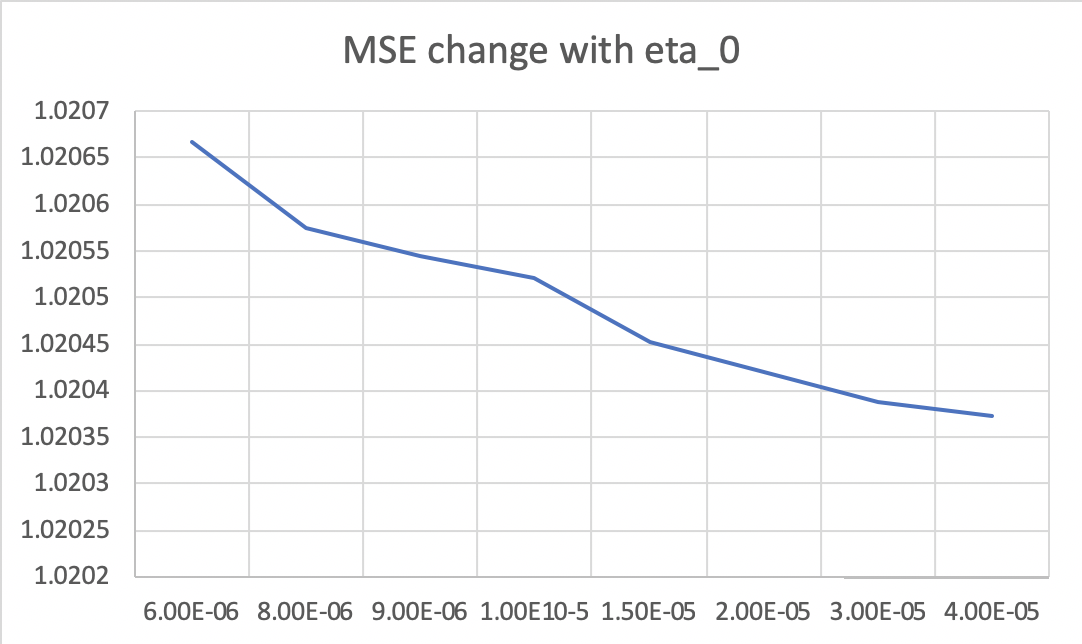
\includegraphics[width=8.5cm, height=5.3cm]{eta0.png}
\\
From the table we find that as the value of $eta_0$ increasing, the value MSE is decreasing, the value $eta_0$= 4.00E-05 has the smallest MSE comparing with other $eta_0$ values, which is 1.020371954.\\
\\
Then we fix $eta_0$ = 4e-05, $beta$ = 0, and change the $eps$ value:\\ 
\\
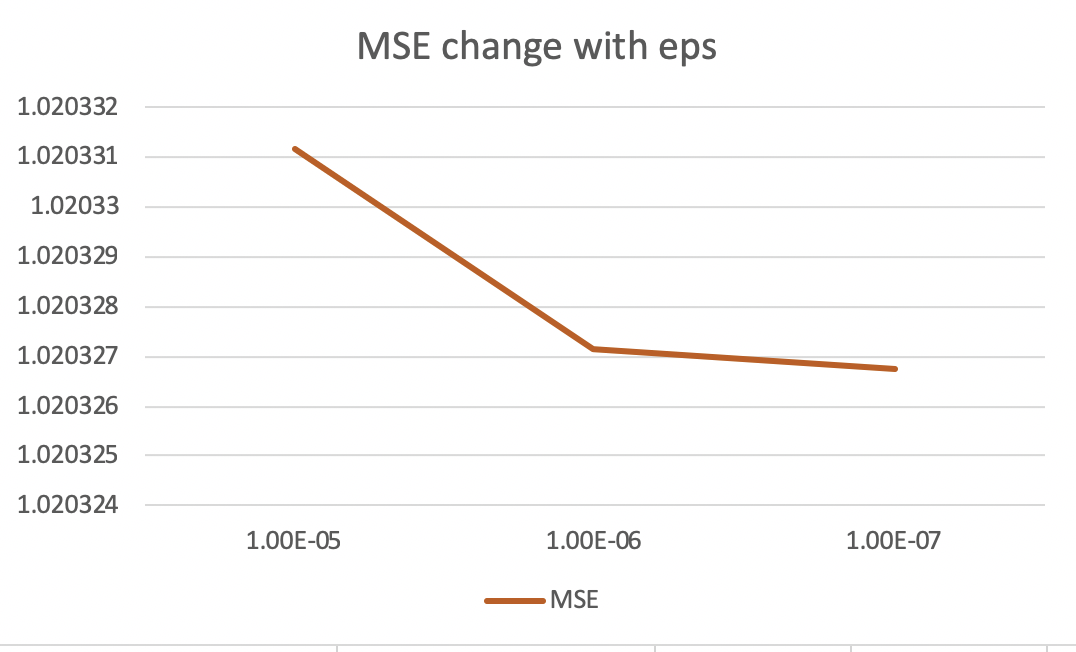
\includegraphics[width=8.5cm, height=5.3cm]{eps.png}
\\
We can see the MSE decreases as the $eps$ value becomes smaller, but the rate of decreasing slows down as $eps$ becomes too small.
\\
Finally we fix $eta_0$ = 4e-05, $beta$ = 0,  $eps$=1e-07, and we try to change the scale of the learning rate $alpha$:
\\
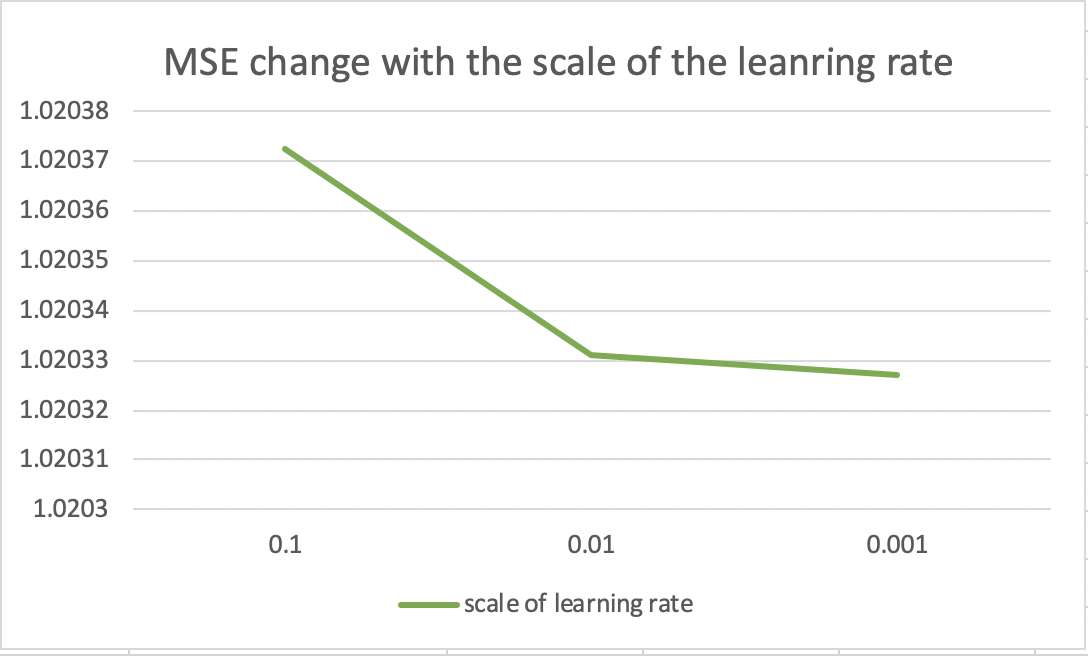
\includegraphics[width=8.5cm, height=5.3cm]{learnrate.png}
\\
As we observe above, the scaling of the learning rate do improve the value of MSE, but just in a very small extent in our experiment, if we change the learning rate to a smaller value, the model seems to fit the data better.\\
\\
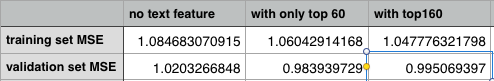
\includegraphics[width=8.5cm, height=1.5cm]{MSE.png}
\\
From the data above, we can see the model with 163 features is over fitting and the model with 3 features is under fitting. We can see the MSE of 63 features is the smallest in validation set. In other words,63 features model is the best prediction of the situation. In the contrast,3 features model has too few features and 163 features model has too much features. Therefore both of their prediction is not as accurate as 63 features model.\\
\\
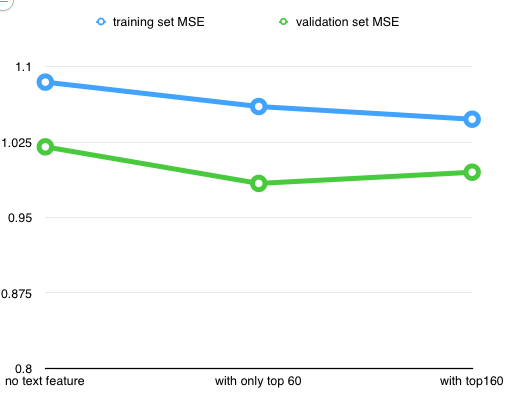
\includegraphics[width=8.5cm, height=6cm]{Graph.png}
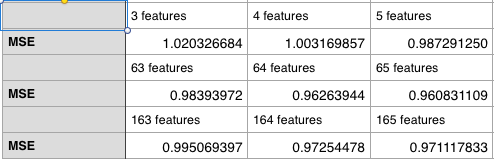
\includegraphics[width=8.5cm, height=3cm]{G.png}
\\
From the table above, we can see that the MSE decrease dramatically for no matter 3,4,5 features or 63,64,65 features or 163,164,165 features.\\
\\
\section{Discussion and Conclusion}
In this study, we have outlined a machine learning workflow that uses linear regression to predict the Reddit comments popularity score. Main takeaways are \textbf{that .....}.
\\
The study discussed in this report could definitely be improved. Possible directions for future improvements include: 
\begin{itemize}
    	\item \textbf{A)} Try out different machine learning models and ensembling methods for better performance
   	\item \textbf{B)} Obtain additional features directly from Reddit (e.g. parent score, whether comment is gilded, a time lapse feature between comments or since root comment was created, etc.)
    	\item \textbf{C)} Remove punctuations from text words.
 	\item \textbf{D)} Assess benefit of removing stop words (e.g. "the", "a", "an", "in") that may no be effective for distinguishing popular comments than non popular ones. 
	\item \textbf{E)} Identify most frequent 2-gram and 3-gram sequences of words and assess whether the model performance can be improved using these.
\end{itemize}

\section{Statement of Contributions}
\begin{itemize}
    	\item \textbf{J-S Grondin} Primary role was to implement the linear regression algorithms and building the machine learning pipeline for this project. Also was responsible for undertaking the exploratory data analysis which led to the selection of additional features. Finally, contributed to the writing of the report. 
   	\item \textbf{Z. Li} ...
    	\item \textbf{Z. Han} ...
\end{itemize}


\end{document}


